\documentclass[12pt]{article}
\usepackage[letterpaper, left=0.5in, top=0.5in, right=0.5in, bottom=1in,nohead,nofoot, verbose, ignoremp]{geometry}
\usepackage{amsmath}
\usepackage{url}

%% Document starts here ...
%%


%opening
\setlength{\parindent}{0pt}

\begin{document}
\vspace{-1in}
\title{\bf STA663 Statistical Computation Final Project}
\author{\bf Implementation of the Indian Buffet Process}
\date{Christine P. Chai}
%\date{\today}
\maketitle 
%\thispagestyle{empty}
\vspace{-0.5in}

%\section{Introduction}
 \section{Introduction}
 \label{sec:intro}
 
% Background -- Situation, Problem, Solution, Evaluation (SPSE)
The paper I selected is ''Infinite Latent Feature Models and the Indian Buffet Process'' (IBP)~\cite{griffiths2005infinite}. In unsupervised machine learning, discovering the hidden variables that generate the observations is important. Many statistical models~\cite{blei2003latent, gershman2012tutorial} can provide a latent structure in probabilitistic modeling, but the problem lies in the unknown dimensionality, i.e. how many classes/features to express the latent structure. Bayesian nonparametric methods are able to determine the number of latent features; the Chinese Restaurant Process (CRP) is an example~\cite{crp2004hierarchical}, but it assigns each customer to a single component (table). The Indian Buffet Process allows each customer to be assigned to multiple components (dishes), and the process can serve as a prior for an potentially infinite array of objects. In my implementation, IBP is regarded as a prior for the linear-Gaussian binary latent feature model, and I referred to some Matlab code online~\cite{ibp2012matlab, ibp2012code}.

\subsection{Algorithm Description}
\label{sub:IBPalg}
The Indian Buffet Process is a metaphor of Indian restaurants offering buffets with a close-to-infinite number of dishes, and the number of dishes sampled by a customer is a Poisson distribution. Assume $N$ customers enter a restaurant one after another, and the first customer takes a Poisson($\alpha$) of dishes. Starting from the second person, the $i$th customer takes dish $k$ with probability $\frac{m_k}{i}$, where $m_k$ is the number of previous customers who have sampled that dish. In this way, the $i$th customer samples dishes proportional to their popularity. After reaching the end of all previously sampled dishes, the $i$th customer tries a Poisson($\frac{\alpha}{i}$) number of new dishes. Which customer sampled which dish is recorded in a binary array $Z$ with $N$ rows (representing customers) and infinitely many columns (representing dishes), where $z_{ik} = 1$ if customer $i$ sampled the dish $k$. Note that the customers are not exchangeable, i.e. the dishes a customer samples is dependent on whether previous customers have sampled that dish~\cite{griffiths2005infinite}.\\ 

In terms of probability, 
\begin{equation}
P(z_{ik}=1 | \mathbf{z_{-i,k}}) = \displaystyle \frac{m_{-i,k}}{N}
\end{equation}
The subscript $\mathbf{_{-i,k}}$ indicates dish $k$ and all customers except for the $i$th one. If the number of dishes is truncated to $K$, then the above equation becomes
\begin{equation}
P(z_{ik}=1 | \mathbf{z_{-i,k}}) = \displaystyle \frac{m_{-i,k} + \frac{\alpha}{K}}{N + \frac{\alpha}{K}}
\end{equation}

% Write the equations here, so we do not need to write in the code structure
The $N$ customers can be viewed as objects, and the $K$ dishes can be regarded as features. Formally writing, $Z \sim \text{IBP}(\alpha)$, and
\begin{equation}
P(Z | \alpha) = \dfrac{\alpha^K}{\prod^{2^N-1}_{h=1}K_h!} \exp(-\alpha H_N) \prod^{K}_{k=1}\dfrac{(N-m_k)!(m_k-1)!}{N!}
\end{equation}
$\alpha$ is a variable influencing the number of features (denoted as $D$ in later sections); $m_k$ is the number of objects with feature $k$; $K_h$ is the number of features with history $h$ (whether the $N$ objects possess this feature, $2^N-1$ possibilities in total); $H_N$ is the $N^{\text{th}}$ harmonic number, i.e. $H_N = \sum^{N}_{k=1}\frac{1}{k}$.

\subsection{Applications and Evaluation}
Many applications and variations of the Indian Buffet Process exist. For example, the linear-Gaussian binary latent feature model I implemented~\cite{ibp2012matlab} can be used to model ''noisy'' matrices and reveal the latent features. In this way, image data can be processed because we can interpret binary matrices with structured representations. For another example, Yildirim and Jacob~\cite{yildirimbayesian} proposed an IBP-based Bayesian nonparametric approach to multisensory perception in an unsupervised manner. Furthermore, variations of the Indian Buffet Process include focused topic modeling~\cite{williamson2009focused}, hierarchical beta processes~\cite{williamson2009focused}, and variational inference~\cite{doshi2008variational}. \\

The advantages and disadvantages of IBP are clear. Using a Poisson distribution, IBP is able to model an infinite sequence of integers, and the sequence can be truncated as needed. In the implementation of IBP, the advantages of Gibbs sampling and Metropolis-Hastings (MH) can be combined. Nevertheless, IBP relies on the assumption that datapoints (dishes) in a single string are exchangeable; each dish is assumed to be equally desired by customers. Another drawback is that the number of parameters increase as the dataset gets large, but Bayesian nonparameteric methods generally have this problem~\cite{ibp2012matlab}.


%\section{Code Structure and Simulated Data}
\section{Code Structure and Simulated Data}
To implement the linear-Gaussian binary latent feature model~\cite{griffiths2005infinite, ibp2012matlab} with IBP as the prior, a Gibbs sampler is used to generate the posterior samples, and the graphical model is shown in Figure~\ref{fig:IBPgeneration}. The IBP function is described in Section~\ref{sub:IBPalg}, and denoted as $Z \sim \text{IBP}(\alpha)$, where $Z$ is the binary matrix and $\alpha \sim Ga(1,1)$.

\begin{figure}
\centering
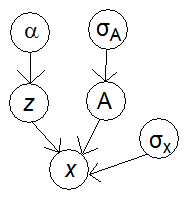
\includegraphics[width=0.25\linewidth]{More_Images/IBP_generation.png}
\caption {Graphical model for the linear-Gaussian binary latent feature model}
\label{fig:IBPgeneration}
\end{figure}

\subsection{Simulated Data for Likelihood}
\label{sub:simulated}

The likelihood involves simulated image data, and the variables are defined as follows:

\begin{itemize}
\item $N = 100$ is the number of images (customers or objects)
\item $D = 6 \times 6 = 36$ is the length of vectors (dishes or features) for each image
\item $K = 4$ is the number of basis images (latent or underlying variables)
\item $\mathbf{X}$ represents the images generated by the $K$ bases (each basis is present with probability 0.5), with white noises $\text{Normal}(0,\sigma_X^2 = 0.5^2)$ added
\end{itemize}

The likelihood function is
\begin{gather}
\mathbf{X}|(\mathbf{Z},\mathbf{A},\mathbf{\sigma_X}) \sim \text{Normal}(\mathbf{ZA},\Sigma_X = \sigma_X^2\mathbf{I}) \\
P(\mathbf{X} | \mathbf{Z}, \sigma_X, \sigma_A) = \dfrac{1}{(2\pi)^{ND/2} \sigma_X^{(N-K)D} \sigma_A^{KD} |\mathbf{Z}^T\mathbf{Z} + \dfrac{\sigma_X^2}{\sigma_A^2}\mathbf{I}|^{D/2}} \exp\{-\dfrac{1}{2\sigma^2_X} \text{tr}(\mathbf{X}^T(\mathbf{I}-\mathbf{Z}(\mathbf{Z}^T\mathbf{Z}+\dfrac{\sigma_X^2}{\sigma_A^2}\mathbf{I})^{-1}\mathbf{Z}^T)\mathbf{X})\}
\end{gather}

Each object $i$ has a $D$-dimensional vector of properties named $x_i$, where:
\begin{itemize}
\item $x_i \sim \text{Normal}(\mathbf{z_i} \mathbf{A}, \Sigma_X = \sigma_X^2\mathbf{I})$
\item $\mathbf{z_i}$ is a $K$-dimensional binary vector (features)
\item $\mathbf{A}$ is a $K \times D$ matrix of weights, with prior $\mathbf{A} \sim \text{Normal}(0,\sigma_A^2 \mathbf{I})$
\end{itemize}

% Need to generate the images here :)
The four basis images and an example of the simulated data are shown in Figure~\ref{fig:images}. Note that the likelihood involves close-to-zero probabilities, so the log likelihood is used in my code instead.

\begin{figure}[!ht]
\centering
    \begin{minipage}{0.8\linewidth}
    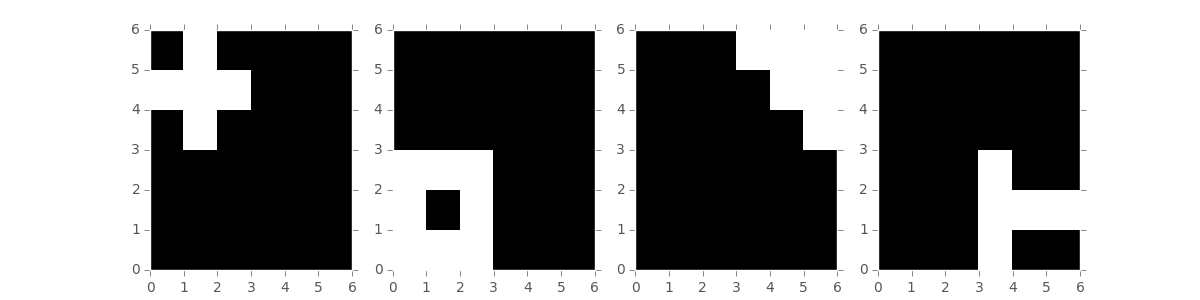
\includegraphics[width=\linewidth]{Version0_Wrong/basis_images.png}
    %\caption{The four basis images}
    %\label{fig:basis}
    \end{minipage}%
    \begin{minipage}{0.2\linewidth}
    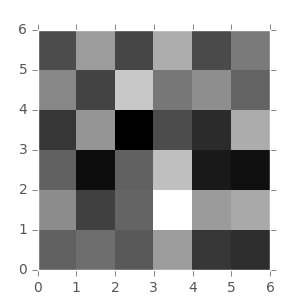
\includegraphics[width=\linewidth]{Version0_Wrong/example_image.png}
    %\caption{An example image}
    %\label{fig:example}
    \end{minipage}
    \caption{Simulated dataset: The four basis images (left) and an example image (right)}
    \label{fig:images}
\end{figure}

\subsection{Gibbs Sampler for the Posterior Distribution}

The full (posterior) conditional distribution is
\begin{equation}
P(z_{ik} | \mathbf{X,Z_{-i,k}},\sigma_X, \sigma_A) \propto P(\mathbf{X} | \mathbf{Z_{-i,k}},\sigma_X, \sigma_A) P(z_{ik} | \mathbf{z_{-i,k}})
\end{equation}

When initializing the Gibbs sampler, set $\sigma_A = 1, \sigma_X = 1, \alpha \sim Ga(1,1)$. Then the sampler does the following steps: ($K$ in my code is denoted as $K_+$, to differentiate it from the true value.)

\begin{enumerate}
\item Generate $P(z_{ik} | \mathbf{X,Z_{-i,k}},\sigma_X, \sigma_A)$ using the full conditional distribution
    \begin{enumerate}
    \item Remove singular features (at most one object has it);\\
    decrease $K_+$ by 1 for each feature removed
    \item Determine each $z_{ik}$ to be $0$ or $1$ by Metropolis
    \item Add new features from $\text{Pois}(\frac{\alpha}{i})$
    \end{enumerate}
\item Sample $\sigma_{X}^* = \sigma_X + \epsilon$, where $\epsilon \sim \text{Unif}(-0.05,0.05)$, and accept $\sigma_{X}^*$ by Metropolis 
\item Sample $\sigma_{A}^* = \sigma_A + \epsilon$, where $\epsilon \sim \text{Unif}(-0.05,0.05)$, and accept $\sigma_{A}^*$ by Metropolis 
\item Generate $\alpha|Z \sim Ga(1+K_+,1+\sum^{N}_{i=1}H_i)$, where $K_+$ is the number of features with $m_k > 0$
\end{enumerate}

The Metropolis part for $\sigma_A$ is demonstrated as follows (similar case for $\sigma_X$):
\begin{itemize}
\item Genenerate a candidate value $\sigma_{A}^{*} = \sigma_{A} + \epsilon$, with $\epsilon \sim \text{Unif}(-0.05,0.05)$
\item Generate a random number $r \sim \text{Unif}(0,1)$
\item Accept $\sigma_{A}^{*}$ if $r < \text{min}\{ 1, \dfrac{P(\sigma_{A}^{*} | \mathbf{Z,X},\sigma_X)}{P(\sigma_{A} | \mathbf{Z,X},\sigma_X)} \}$, where $\sigma_{A}$ is the current value
\end{itemize}

The candidate value $\sigma_{A}^{*}$ is always accepted when the likelihood ratio $\frac{P(\sigma_{A}^{*} | \mathbf{Z,X},\sigma_X)}{P(\sigma_{A} | \mathbf{Z,X},\sigma_X)}$ is larger than 1, i.e. $P(\sigma_{A}^{*} | \mathbf{Z,X},\sigma_X) > P(\sigma_{A} | \mathbf{Z,X},\sigma_X)$. Nevertheless, when the likelihood ratio is less than 1, there is still a non-zero probability to accept $\sigma_{A}^{*}$, so the sampler can ''move forward''. Note that in my code, the log likelihoods are used in the following way:

% including how to normalize the log/relative probabilities
\begin{equation}
\text{min}\{ 1, \dfrac{P(\sigma_{A}^{*} | \mathbf{Z,X},\sigma_X)}{P(\sigma_{A} | \mathbf{Z,X},\sigma_X)} \} = \exp(\text{min}\{0, \log(P(\sigma_{A}^{*} | \mathbf{Z,X},\sigma_X)) - \log(P(\sigma_{A} | \mathbf{Z,X},\sigma_X))\})
\end{equation}

Finally, the posterior expectation of $\mathbf{A}$ is:
\begin{equation}
E(\mathbf{A}|\mathbf{X,Z}) = (\mathbf{Z}^T\mathbf{Z}+\frac{\sigma_X^2}{\sigma_A^2}\mathbf{I})^{-1} \mathbf{Z}^T \mathbf{X}
\end{equation}
This is denoted as $\mathbf{A}_{\text{inf}}$, with size $D \times K_+$, and $\mathbf{A}_{\text{inf}}$ is the matrix of latent features (images) my code converges to.

\section{Testing}

\section{Optimization}

\subsection{Remove Redundant Calculations}

\subsection{Cythonized Code}

\section{Comparative Analysis}

\subsection{Chinese Restaurant Process}

\subsection{Another Matlab Version Online}

\subsection{Another Python Version Online}

\section{Results}

Table~\ref{tbl:hit} shows a simple version of tables.

%\begin{minipage}{\textwidth} % Don't add minipage in front of tables!
\begin{table}
  \centering
  \begin{tabular}{rr}
\hline
    dog &    cat \\
\hline
 2.0000 & 3.0000 \\
 4.0000 & 7.0000 \\
 5.0000 & 8.0000 \\
\hline
\end{tabular}
  \caption{Our top noise discoveries.}
  \label{tbl:hit}
\end{table}
%\end{minipage}


%Figure~\ref{fig:heatmap}.

%\begin{figure}
%\includegraphics[width=\linewidth]{heatmap.png}
%\caption {Heatmap showing noise discovery in case-control studies.}
%\label{fig:heatmap}
%\end{figure}


\section{Conclusion}

Write your conclusion here

\bibliographystyle{plain}
\bibliography{intro}


\end{document}